%%%%%%%%%%%%%%%%%%%%%%%%%%%%%%%%%%%%%%%%%%%%%%%%%%%%%%%%%%%%%%%%%%%%%%%%%%%%%%%%
%% 
\cleardoubleoddpage%  Make sure to start each chapter on a new odd page
\chapter{Literature Review}

\section{Current State of Respiratory Sound Analysis}
Lung auscultation is the standard method of diagnosing respiratory disease by listening to the patient's lungs through the chest. However, this approach, which relies on manual assessment by healthcare professionals, has several limitations. Its effectiveness depends on the physician's skill, experience, and auditory sensitivity, leading to potential inaccuracies in diagnosis~\cite{palaniappan2013computer}. In addition, manual auscultation is typically limited to clinical settings, missing critical auditory cues that may occur outside of these settings, such as nocturnal breath sounds common in conditions such as asthma~\cite{pramono2017automatic}. \\
These limitations, combined with technological advances, have led to the development of computerized respiratory sound analysis. In this approach, lung sounds are digitally recorded and then analyzed. Early techniques focused on the graphical representation of sound waves, allowing medical professionals to identify abnormalities visually. However, this method did not fully mitigate the risk of human error. Subsequently, statistical approaches were developed to assess the frequency of specific respiratory events based on historical data patterns. According to systematic reviews~\cite{palaniappan2013computer}, machine learning-based approaches provide the most promising results but were limited by the need for sufficiently large data sets.

\subsection{The ICBHI Challenge 2017}
During the 2017 Annual International Conference on Biomedical and Health Informatics, a central challenge was launched in response to the scarcity of comprehensive lung sound data. This challenge aimed to foster the development and evaluation of advanced algorithms for automated lung sound classification using a novel dataset curated specifically for this purpose. Known as the Respiratory Sound Database~\cite{rocha2018alpha}, this collection stands out as one of the field's earliest and most comprehensive publicly available datasets, comprising 6.898 respiratory cycles from 126 patients. These recordings, collected by professional teams in Greece and Portugal, represent diverse audio samples, capturing sounds from healthy individuals and patients suffering from lung diseases such as COPD, asthma, and bronchiectasis. Each breathing cycle in the database is annotated by domain experts and categorized as normal, with wheezes, crackles, or both wheezes and crackles. The challenge encouraged many submissions, showcasing a range of innovative machine-learning approaches. Below, we compare a selection of these methods.

\subsection{Existing Approaches}
Starting with traditional artificial intelligence methods, Jakovljevi{\'c} and Lon{\v{c}}ar-Turukalo (2018) published their work based on hidden Markov models (HMM) alongside the paper introducing the Respiratory Sound Database~\cite{jakovljevic2018hidden}. Using MFCCs as features, they employed a four-class classifier with the official 60/40 split at the recording level, using 60\% of the data for training and the remaining 40\% for evaluation. The four classes were healthy, crackles, wheezes, both crackles and wheezes. A Balanced Accuracy score of 0.39 was achieved, with a sensitivity of 0.38 and a specificity of 0.41.\\
Chambres et al. (2018) used boosted decision trees (BDT) to address the four-class classification task~\cite{chambres2018automatic}. They used the same 60/40 split and MFCCs as features. The model architecture significantly improved the balance accuracy to 0.49, with a sensitivity of 0.78 and a specificity of 0.21.\\
Shortly after, the use of neural networks gained traction. Ma et al. (2019) proposed the use of a bi-ResNet (LungBRN) architecture~\cite{wang2019bi} consisting of multiple concatenated convolutional neural network layers~\cite{ma2019lungbrn}. Using the same split as the other approaches but short-time Fourier transform (STFT) and wavelet analysis to extract features, they achieved an official Balanced Accuracy of 0.5, specificity of 0.69, and sensitivity of 0.31 for the four-class problem.\\
The Microsoft Research India team around Gairola et al. (2021) published their RepireNet~\cite{gairola2021respirenet} network and benchmarked it in various data splits and binary and four-class classification problems. The backbone is blocks of ResNet34~\cite{he2016deep} deep convolutional neural networks (CNN). Using MelSpectrograms as features, their baseline CNN achieved 0.55 Balanced Accuracy on the official 60/40 split, 0.66 Balanced Accuracy for the four-class problem on a self-defined random 80/20 split at the breathing cycle level, and 0.72 on the same 80/20 split but treating the problem as a binary classification, which allows for an easier comparison to a anomaly detection setting.\\
\begin{table}[h!]
    \centering
    \caption{
        Performance comparisons of the showcased models 
    }
    \begin{tabularx}{\linewidth}{lXcccc}
    \toprule
    \textbf{Model}        & \textbf{Split} & \textbf{Features} & \textbf{Se} & \textbf{Sp} & \textbf{BALACC} \\
    \midrule
    HMM                   & 60/40 4 class          & MFCC              & 0.38                & 0.41                 & 0.39 \\
    BDT                   & 60/40 4 class          & MFCC              & 0.78                & 0.21                 & 0.49 \\
    LungBRN               & 60/40 4 class          & STFT + Wavelet    & 0.69                & 0.31                 & 0.5  \\
    RespireNet CNN        & 60/40 4 class          & MelSpectrogram    & 0.39                & 0.71                 & 0.55 \\
    RespireNet CNN        & 80/20 4 class  & MelSpectrogram    & 0.54                & 0.79                 & 0.66 \\
    RespireNet CNN        & 80/20 2 class  & MelSpectrogram    & 0.61                & 0.83                 & 0.72 \\
    \bottomrule
    \end{tabularx}
\end{table}
    
It is important to note that all mentioned respiratory sound analysis approaches rely on treating it as a supervised classification task. While effective in their context, these methods assume the availability of extensive labeled data representing various specific respiratory conditions. However, such comprehensive data sets are rarely readily available in real-world scenarios. Furthermore, the strict categorization of respiratory sounds into predefined classes may overlook respiratory anomalies' nuanced and unpredictable nature. Therefore, the remainder of this thesis will explore respiratory sound analysis through the lens of anomaly detection.

\section{Respiratory Sound Analysis from an Anomaly Detection Perspective}
Using anomaly detection methods to solve sound analysis problems is not new. In particular, these methods have proven their effectiveness in industrial sound analysis, as demonstrated in Task 2 of the annual DCASE Challenge~\cite{dcaseDCASE2023Challenge}, where machine condition monitoring is performed by observing the sound produced by these machines. The sound emitted can be either normal or anomalous, and machine learning algorithms learn to understand the characteristics of healthy machine sounds to accurately predict machine failure in the case of anomalous sounds such as rattling or whirring.\\
A similar approach can be used in breathing sound analysis. The different anomalous respiratory sounds can all be grouped into a single anomaly class, and anomaly detection models can learn the constitution of healthy respiratory cycles. If a sample deviates significantly from the learned representation of a healthy sound, the system can flag it as anomalous.


\section{Variational Autoencoders}
Cozzatti et al. (2022)~\cite{cozzatti2022variational} explored the first anomaly detection approach to the respiratory sound database. Their work used MFCCs as features, and the breathing cycles containing wheezes, crackles, or both were all summarized in an anomaly class. A Variational Autoencoder (VAE) was trained using only known healthy breathing cycles.\\
Variational Autoencoders are similar to Autoencoders, consisting of an encoder and a decoder part (\autoref{fig:archvae}). By comparison, the encoder of a VAE uses variational inference to output the parameters of a continuous and easily sampled distribution, usually the mean and standard deviation of a  Gaussian~\cite{cozzatti2022variational}. As a result, the input to the decoder is a single sample from that predicted distribution. VAEs still rely on the reconstruction error between the input to the encoder and the decoder output. However, they can use the variability of the stochastic latent space for the sampling in the decoder, providing a measure of certainty of the reconstructed data~\cite{an2015variational}.\\

\begin{figure}[h!]
    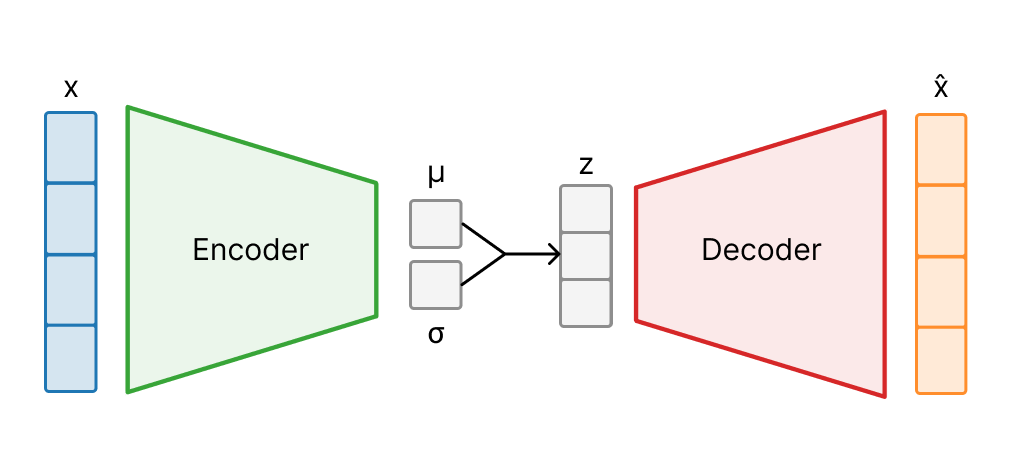
\includegraphics[width=\linewidth]{images/vae}
    \caption{
    Architecture of VAE, sampling into latent space z from Gaussian distribution
}
\label{fig:archvae}
\end{figure}


Training the VAE with normal sounds only teaches it to reconstruct physiological respiratory cycles accurately. The reconstruction error reported by the model is small in this case. When the model attempts to reconstruct a respiratory sound with pathologies, the parameters of the Gaussian will most likely not match the parameters of the learned distribution of healthy sounds. Thus, the reconstruction will have a higher error. The paper then used a small subset of the original dataset containing healthy and unhealthy lung sounds to determine a threshold in the reconstruction error above which all higher errors should be marked as anomalous, making the process weakly supervised. The proposed model achieved competitive results in the binary class problem, with a Balanced Accuracy of 0.57 for the official 60/40 split and 0.6 for a random 80/20 split.

\begin{table}[h!]
    \centering
    \caption{Performance of the proposed method}
    \begin{tabular}{cccccc}
    \toprule
    \textbf{Split} & \textbf{Se} & \textbf{Sp} & \textbf{BALACC} \\
    \midrule
    60/40 & 0.33 & 0.80 & 0.57 \\
    80/20 & 0.58 & 0.61 & 0.60 \\
    \bottomrule
    \end{tabular}
\end{table}


\section{Group Masked Autoencoders}
In \autoref{theory:made}, we have discussed how Masked Autoencoders are an alternative anomaly detection approach to generative models by evaluating probability densities. The basic concept focused on modifying an existing autoencoder structure to satisfy the autoregressive property by masking the weights of the neural network layers so that each output dimension depends only on the preceding input dimensions.\\
When working with sound data representations such as MelSpectrograms or MFCCS, the focus shifts from the autoregressive ordering of individual input dimensions to the ordering of sound frames. Here, Group Masked Autoencoders (GMADE)~\cite{Giri2020} provide a more tailored approach for audio anomaly detection tasks where temporal context is important. GMADE differs from traditional MADE in that it does not split the joint distribution into individual dimensional conditions but rather into conditionals on the grouped frames. This approach is particularly relevant when dealing with sound data, where each time frame in a MelSpectrogram is considered a separate group.\\
In GMADE, the input space has the dimensionality $T\times M$, where $T$ is the number of frames concatenated in the input and $M$ is the number of Mel frequency bands. If an input sample can be thought of as $\mathbf{t}=[\mathbf{t_{i+1}}, \mathbf{t_{i+2}},... ,\mathbf{t_{i+T}}]$ with $\mathbf{t_{i}}\in \mathbb{R}^{M\times 1}$, the joint density can be decomposed as \[ p(\mathbf{t})=\sum_{i=1}^{T}p(\mathbf{t_i}|\mathbf{t}_{<i}) \] where the probability of each frame depends on all previous frames and their mel bins and no other frames~\cite{Giri2020}. To maintain the autoregressive property, the generation of the weight matrices must be slightly adapted from the MADE approach to assign labels to the neurons only from $1$ to $T-1$ to correctly zero out connections between groups instead of units.\\
The paper also explored orderings other than causal, where a frame can only depend on its predecessors. Backward ordering predicts the probability density of frames given only their succeeding frames, while middle frame ordering attempts to predict the middle frame given only the frames surrounding it. Ensembles of all three approaches were also evaluated. GMADE achieved state-of-the-art results in Task 2 of the DCASE Challenge 2020 in the machine condition monitoring task, especially for non-stationary sounds. While this is promising for respiratory sound analysis due to the non-stationary nature of lung sounds, the efficacy of GMADE in detecting anomalies in respiratory sounds is yet to be tested.\\

We highlighted the significant progress in respiratory sound analysis, moving from traditional auscultation to advanced computational methods. Developing the Respiratory Sound Database has been an important catalyst, enabling the application of machine learning methods in this domain. Notably, the ICBHI Challenge 2017 provided a platform for showcasing diverse approaches, ranging from hidden Markov models and boosted decision trees to more advanced neural network architectures like LungBRN and RespireNet.\\
The shift towards anomaly detection methods marks a transition in the approach towards the dataset. Cozzatti et al. (2022) introduced a novel approach using Variational Autoencoders (VAE), demonstrating the potential of reconstruction-based models in identifying respiratory anomalies. Focusing solely on normal respiratory cycles for training, this method distinguishes abnormal sounds based on the deviation in reconstruction error, achieving notable results in binary classification tasks.\\
Building upon these insights, we will next explore and compare two approaches to respiratory sound analysis: reconstruction-based methods, represented by VAE, and density-estimation-based approaches, represented by Group Masked Autoencoders (GMADE). We will reevaluate the VAE for its effectiveness in distinguishing between normal and pathological respiratory sounds and assess GMADE's ability to accurately model the probability densities of respiratory sounds.

%% 
%%%%%%%%%%%%%%%%%%%%%%%%%%%%%%%%%%%%%%%%%%%%%%%%%%%%%%%%%%%%%%%%%%%%%%%%%%%%%%%%